% !TEX root = main.tex
% !TEX program = pdflatex
% !TEX spellcheck = es_ES
\documentclass[12pt,letterpaper]{article}

\usepackage[spanish,es-tabla]{babel}
\usepackage[utf8]{inputenc}
\usepackage[T1]{fontenc}
\usepackage{amsmath}
\usepackage{newtxtext,newtxmath}
\usepackage{geometry}
\usepackage{booktabs}
\usepackage{longtable}
\usepackage{tabularx}
\usepackage{array}
\usepackage{listings}
\usepackage{xcolor}
\usepackage{needspace}
\usepackage{titlesec}
\usepackage{etoolbox}
\usepackage[protrusion=true,expansion=false]{microtype}
\usepackage[all]{nowidow}
\usepackage{enumitem}
\usepackage[section]{placeins}
\usepackage{graphicx}
\usepackage{float}
\usepackage{subcaption}
\usepackage{caption}
\usepackage{tikz}
\usepackage{pgfplots}
\usepackage{pgfplotstable}
\usepackage{fancyhdr}
\usepackage[font=small,labelfont=bf]{caption}
\usepackage{hyperref}
\usepackage{natbib}
\usepackage{csquotes}

\geometry{margin=2.5cm}
\hypersetup{colorlinks=true,linkcolor=black,citecolor=black,urlcolor=blue,pdfborder={0 0 0}}
\setlength{\parskip}{0.6em}
\setlength{\parindent}{0pt}
\raggedbottom

\pgfplotsset{compat=1.18}
\usetikzlibrary{arrows.meta,positioning,shapes.geometric,calc,fit,backgrounds}

% Paleta cromatica del proyecto Mineria de Datos
\definecolor{dmTeal}{HTML}{0F766E}
\definecolor{dmInk}{HTML}{172033}
\definecolor{dmLine}{HTML}{D6DEE8}
\definecolor{dmMuted}{HTML}{5B667A}
\definecolor{dmAdelie}{HTML}{1F77B4}
\definecolor{dmChinstrap}{HTML}{D97706}
\definecolor{dmGentoo}{HTML}{16A34A}
\definecolor{dmAccent}{HTML}{0B2E4F}

% =====================================================================
%  CONTROL DE SALTOS DE PAGINA (estandar academico, totalmente automatico)
%  Objetivo: ningun parrafo, titulo de seccion, lista o figura se rompa
%  visualmente mal entre paginas. La combinacion de penalizaciones y de
%  \Needspace antes de cada titulo garantiza que el motor de LaTeX:
%    1. Nunca deje viudas (ultima linea de un parrafo en pagina nueva).
%    2. Nunca deje huerfanos (1ra linea de un parrafo al pie de pagina).
%    3. Nunca rompa una palabra con guion al final de pagina.
%    4. Nunca coloque un titulo de seccion en las ultimas lineas de
%       la pagina sin al menos N lineas de contenido debajo.
%    5. No separe figuras/listas/displays de su contexto.
%  La tolerancia tipografica adicional evita overfull cuando las
%  penalizaciones altas obligan a recomponer parrafos.
% =====================================================================

% --- (1) Penalizaciones de ruptura ---
\clubpenalty=10000                  % huerfano: 1ra linea de parrafo al pie
\widowpenalty=10000                 % viuda: ultima linea de parrafo en cima
\displaywidowpenalty=10000          % idem para entornos display
\predisplaypenalty=10000            % no romper inmediatamente antes de un display
\postdisplaypenalty=0               % permitir respirar tras un display
\brokenpenalty=10000                % no romper pagina en linea con guion
\interlinepenalty=200               % suave: desincentiva ruptura en mitad de parrafo

% --- (2) Espaciado de titulos (titlesec) ---
\titlespacing*{\section}{0pt}{1.4em}{0.6em}
\titlespacing*{\subsection}{0pt}{1.0em}{0.4em}
\titlespacing*{\subsubsection}{0pt}{0.8em}{0.3em}

% --- (3) \Needspace antes de cada titulo ---
% Si quedan menos lineas que el umbral, el motor fuerza un salto de pagina
% ANTES del titulo, garantizando que cada seccion arranque con suficiente
% contenido visible debajo (evita titulos huerfanos al pie de pagina).
\pretocmd{\section}{\Needspace{14\baselineskip}}{}{}
\pretocmd{\subsection}{\Needspace{9\baselineskip}}{}{}
\pretocmd{\subsubsection}{\Needspace{7\baselineskip}}{}{}
\pretocmd{\paragraph}{\Needspace{5\baselineskip}}{}{}

% --- (4) Barrera de flotantes por seccion (placeins ya cargado) ---
% Refuerza que las figuras no migren a la siguiente seccion.
\pretocmd{\section}{\FloatBarrier}{}{}

% --- (5) Listas: forzar que el primer item siga al texto introductorio ---
\AtBeginEnvironment{itemize}{\par\nopagebreak}
\AtBeginEnvironment{enumerate}{\par\nopagebreak}
\AtBeginEnvironment{description}{\par\nopagebreak}

% --- (6) Tolerancia tipografica ---
% Con penalizaciones tan altas, el motor puede no encontrar saltos validos
% y generar overfull boxes. Aflojamos la tolerancia y damos margen de
% estiramiento de emergencia para que recomponga parrafos sin desbordes.
\tolerance=600
\emergencystretch=3em

% --- (7) Tablas y longtable ---
\setlength{\LTpre}{0.25em}
\setlength{\LTpost}{0.6em}
\renewcommand{\arraystretch}{1.08}
\newcolumntype{P}[1]{>{\raggedright\arraybackslash}p{#1}}
\newcolumntype{C}[1]{>{\centering\arraybackslash}p{#1}}
\setlist{topsep=0.25em,itemsep=0.15em,parsep=0pt}
\BeforeBeginEnvironment{longtable}{\Needspace{10\baselineskip}\small}
\AfterEndEnvironment{longtable}{\normalsize}

% --- (7b) Listings de codigo ---
% Los bloques lstlisting pueden romperse entre paginas si no hay espacio
% suficiente, dejando codigo cortado a la mitad (poco profesional en
% reportes academicos). Reservamos al menos 14 lineas de pagina antes
% de emitir un listing: si quedan menos, el motor lo empuja a la pagina
% siguiente, garantizando que el listing inicie limpio.
\BeforeBeginEnvironment{lstlisting}{\par\Needspace{14\baselineskip}}

% --- (8) Control de saltos dentro del INDICE (\tableofcontents) ---
% Problema: el motor de LaTeX puede romper el TOC entre una seccion y sus
% subsecciones porque la glue entre entradas es un candidato libre de
% ruptura. Solucion en tres frentes (ninguno basta por si solo):
%   (a) Reducir el espaciado vertical entre entradas de seccion en el TOC
%       de 1.0em a 0.4em, asi entran mas entradas por pagina (compresion).
%   (b) Anular \parskip dentro del TOC: elimina la glue \par que separa
%       entradas y que era el principal candidato de ruptura.
%   (c) Redefinir \l@section para emitir \penalty\@highpenalty AL FINAL
%       de cada entrada de seccion, prohibiendo el salto inmediato.
%   (d) Inyectar \nobreak antes de cada subseccion como refuerzo.
\makeatletter
% Reglas TeX de ruptura en vmode:
%   - Una glue es punto de ruptura valido SOLO si el nodo previo no es
%     descartable (penalty/glue son descartables; cajas/rules no).
%   - penalty -10000 = ruptura FORZADA (no la queremos). Usamos \@secpenalty
%     (=-300) que es la convencion academica para "preferir romper aqui".
%   - penalty +10000 = ruptura PROHIBIDA en ese nodo (la queremos tras el
%     titulo de seccion para mantenerlo pegado a sus subsecciones).
% Para que la penalty alta sea efectiva:
%   1) \removelastskip elimina la glue residual de \par.
%   2) \penalty\@M crea un nodo de penalty alta.
%   3) La glue inicial de la siguiente subseccion (precedida por penalty)
%      deja de ser candidata por la regla "glue tras descartable no rompe".
\renewcommand*\l@section[2]{%
  \ifnum \c@tocdepth >\z@
    \addpenalty{\@secpenalty}%
    \addvspace{0.3em \@plus\p@}%
    \setlength\@tempdima{1.5em}%
    \begingroup
      \parindent \z@ \rightskip \@pnumwidth
      \parfillskip -\@pnumwidth
      \parskip \z@
      \leavevmode \bfseries
      \advance\leftskip\@tempdima
      \hskip -\leftskip
      #1\nobreak\hfil \nobreak\hb@xt@\@pnumwidth{\hss #2}\par
      \removelastskip
      \penalty\@M
    \endgroup
  \fi}
% Subsecciones: penalty alta antes (mantiene cohesion con la seccion
% padre) y despues (entre subsecciones consecutivas no se rompe).
\let\dm@old@l@subsection\l@subsection
\renewcommand*{\l@subsection}[2]{%
  \removelastskip\penalty\@M
  \begingroup\parskip\z@\dm@old@l@subsection{#1}{#2}\removelastskip\penalty\@M\endgroup}
\let\dm@old@l@subsubsection\l@subsubsection
\renewcommand*{\l@subsubsection}[2]{%
  \removelastskip\penalty\@M
  \begingroup\parskip\z@\dm@old@l@subsubsection{#1}{#2}\removelastskip\penalty\@M\endgroup}
\makeatother
% Eliminar parskip en el TOC entero (refuerza la solucion: sin parskip,
% no hay glue entre entradas, asi que tampoco hay candidatos de ruptura
% adicionales).
\AtBeginDocument{%
  \addtocontents{toc}{\protect\setlength{\protect\parskip}{0pt}}%
  \addtocontents{lof}{\protect\setlength{\protect\parskip}{0pt}}%
  \addtocontents{lot}{\protect\setlength{\protect\parskip}{0pt}}%
}
% =====================================================================

\lstset{
  basicstyle=\ttfamily\small,
  breaklines=true,
  frame=single,
  framesep=4pt,
  rulecolor=\color{dmLine},
  backgroundcolor=\color{dmLine!10},
  columns=fullflexible,
  keywordstyle=\color{dmTeal}\bfseries,
  commentstyle=\color{dmMuted}\itshape,
  stringstyle=\color{dmChinstrap},
  showstringspaces=false,
}

\pagestyle{fancy}
\fancyhf{}
\fancyhead[L]{\footnotesize\color{dmMuted}Mineria de Datos -- Clustering Palmer Penguins}
\fancyhead[R]{\footnotesize\color{dmMuted}\leftmark}
\fancyfoot[C]{\footnotesize\color{dmMuted}\thepage}
\renewcommand{\headrulewidth}{0pt}
\renewcommand{\footrulewidth}{0pt}

\title{Clustering No Supervisado del Dataset Palmer Penguins: Comparativa entre K-Means, DBSCAN y Agglomerative}
\author{Samuel Hiram Castro Martinez}
\date{26 de Mayo del 2026}

\begin{document}

\begin{titlepage}
  \centering
  {\Large Instituto Tecnológico de Tijuana\par}
  \vspace{0.4cm}
  {\large Maestría en Ciencias de la Computación\par}
  \vspace{1.6cm}
  {\color{dmTeal}\rule{0.7\linewidth}{1pt}\par}
  \vspace{0.8cm}
  {\LARGE\bfseries Clustering No Supervisado del Dataset Palmer Penguins: Comparativa entre K-Means, DBSCAN y Agglomerative Clustering\par}
  \vspace{0.4cm}
  {\color{dmTeal}\rule{0.7\linewidth}{1pt}\par}
  \vspace{1.6cm}
  \begin{tabularx}{0.92\textwidth}{>{\bfseries}r X}
    Materia: & Minería de Datos\\
    Profesor: & Dr. Mario Garcia\\
    Semestre: & Enero -- Junio 2026\\
    Alumno: & Samuel Hiram Castro Martinez\\
    Matrícula: & 25210035\\
    Programa: & Maestría en Ciencias de la Computación\\
    Proyecto: & Clustering no supervisado sobre Palmer Penguins\\
    Versión: & 1.0 (notebook reproducible con figuras y métricas integradas)\\
    Fecha: & 26 de Mayo del 2026
  \end{tabularx}
  \vfill
  \small\color{dmMuted} Reporte elaborado bajo la práctica de Ciencia 2.0: datos públicos con licencia abierta, código fuente reproducible y semillas aleatorias fijadas.\par
\end{titlepage}

% !TEX root = ../reporte_final.tex
\section*{Resumen ejecutivo}
\addcontentsline{toc}{section}{Resumen ejecutivo}

Este documento reporta una investigación corta de minería de datos sobre el dataset \emph{Palmer Penguins} \citep{horst2020palmer,gorman2014ecological}. Se compara la capacidad de tres algoritmos de clustering no supervisado --- K-Means \citep{macqueen1967some}, DBSCAN \citep{ester1996density} y Agglomerative Clustering con linkage de Ward \citep{ward1963hierarchical} --- para recuperar automáticamente la estructura de especies a partir únicamente de las cuatro variables morfométricas del dataset, sin utilizar la etiqueta de especie durante el entrenamiento.

\paragraph{Aportes principales}
\begin{itemize}
  \item Flujo de minería de datos completo en un único notebook reproducible: definición del problema, obtención de datos, exploración, preprocesamiento, experimentación, evaluación y conclusiones.
  \item Comparación cuantitativa de los tres algoritmos con dos métricas complementarias: \emph{Silhouette Score} (interna) y \emph{Adjusted Rand Index} (externa, contra la etiqueta verdadera de especie) \citep{rand1971objective,hubert1985comparing,rousseeuw1987silhouettes}.
  \item Visualizaciones vectoriales: \emph{pairplot} discriminado por especie, matriz de correlación, método del codo, proyección PCA bidimensional y matriz de confusión.
  \item Práctica plena de Ciencia 2.0: datos con licencia CC-0, código bajo control de versiones, semillas fijadas (\texttt{RANDOM\_STATE=42}), \texttt{requirements.txt} y notebook ejecutable de principio a fin sin intervención manual.
\end{itemize}

\paragraph{Resultado del experimento}
Sobre 342 observaciones limpias del dataset (tras eliminar valores faltantes en las variables numéricas y en la especie), \textbf{Agglomerative Clustering con linkage de Ward} obtiene el mejor ajuste a la estructura biológica conocida, con un \emph{Adjusted Rand Index} de \textbf{0.916}, un \emph{Silhouette Score} de 0.454 y, tras mapear cada cluster a su especie mayoritaria, una \textbf{exactitud del 96.8\,\%} (331/342). K-Means queda muy próximo (ARI=0.793) y DBSCAN, pese a maximizar la métrica interna (Silhouette=0.557), fusiona las especies \emph{Adelie} y \emph{Chinstrap} en un único cluster denso y produce 33 puntos catalogados como ruido, lo que penaliza su ARI a 0.584.

\paragraph{Defensibilidad académica}
El experimento es totalmente reproducible: tanto el notebook como las semillas, los hiperparámetros y los hashes del dataset están versionados en el repositorio del proyecto. La sección~6 incluye la tabla comparativa de métricas y la sección~7 las conclusiones con limitaciones y trabajo futuro. Los apéndices recogen el código fuente esencial y la checklist de reproducibilidad.
\newpage


\tableofcontents
\listoffigures
\listoftables
\newpage

% !TEX root = ../main.tex
\section{Introducción}

La minería de datos articula un conjunto de técnicas computacionales orientadas a descubrir patrones útiles en grandes volúmenes de información, conjugando estadística, aprendizaje automático y visualización \citep{hankamber2011data,witten2016data}. En su modalidad no supervisada, la disciplina busca estructura latente sin disponer de etiquetas: el clustering es su instancia canónica.

El dataset \emph{Palmer Penguins} \citep{horst2020palmer,gorman2014ecological} se ha consolidado como una alternativa moderna al clásico \emph{Iris}, debido a que ofrece características físicas de tres especies de pingüinos (\emph{Adelie}, \emph{Chinstrap} y \emph{Gentoo}) en tres islas del archipiélago Palmer (Antártida). Su tamaño compacto, su licencia abierta y la presencia controlada de valores faltantes y solapamiento entre especies lo convierten en un banco de pruebas ideal para enseñar y comparar algoritmos de clustering en un contexto reproducible.

\section{Planteamiento del problema}

Los enfoques supervisados de clasificación requieren etiquetas, las cuales no siempre están disponibles --- por ejemplo, en biología de campo o en estudios exploratorios. La pregunta de investigación de este proyecto es:

\begin{quote}
\emph{¿Es posible recuperar la estructura natural de las tres especies de pingüinos del archipiélago Palmer a partir únicamente de variables morfométricas (longitud y profundidad del pico, longitud de la aleta y masa corporal) mediante algoritmos de clustering no supervisado, y qué algoritmo lo hace mejor?}
\end{quote}

La hipótesis es que algoritmos sensibles a la geometría global del espacio de características (K-Means y Agglomerative con linkage de Ward) recuperarán mejor la partición real que algoritmos basados puramente en densidad local (DBSCAN), debido a que las especies presentan tamaños de grupo similares y no exhiben densidades drásticamente distintas.

\section{Objetivo general}

Diseñar, ejecutar y reportar un experimento de minería de datos --- siguiendo prácticas de Ciencia 2.0 --- que compare K-Means, DBSCAN y Agglomerative Clustering sobre el dataset Palmer Penguins, evaluando con métricas interna (Silhouette) y externa (Adjusted Rand Index) la calidad de la agrupación obtenida.

\section{Objetivos específicos}

\begin{itemize}
  \item Realizar el análisis exploratorio de datos (EDA) con estadísticas descriptivas, distribución por clase, valores faltantes y correlaciones.
  \item Diseñar un pipeline de preprocesamiento que elimine \texttt{NaN} y estandarice las variables numéricas mediante \texttt{StandardScaler}.
  \item Ajustar y comparar K-Means, DBSCAN y Agglomerative Clustering con hiperparámetros explícitamente documentados.
  \item Calcular y reportar Silhouette Score y Adjusted Rand Index para los tres modelos.
  \item Visualizar los clusters obtenidos sobre la proyección PCA bidimensional y construir la matriz de confusión del mejor algoritmo.
  \item Publicar todos los artefactos (notebook, dataset, requirements, README, presentación, figuras) en un repositorio reproducible.
\end{itemize}

\section{Estructura del documento}

El reporte se organiza en seis secciones principales y dos apéndices. La sección~2 establece el marco teórico de los algoritmos y las métricas. La sección~3 describe la metodología y el pipeline de minería de datos. La sección~4 detalla los experimentos. La sección~5 presenta los resultados con tablas y figuras. La sección~6 concluye con limitaciones y trabajo futuro. El apéndice~\ref{ap:codigo} contiene los fragmentos esenciales de código y el apéndice~\ref{ap:reproducibilidad} la checklist de reproducibilidad de Ciencia 2.0.

% !TEX root = ../reporte_final.tex
\section{Marco teórico}

\subsection{Minería de datos y aprendizaje no supervisado}

La minería de datos se define como el proceso no trivial de extracción de patrones válidos, novedosos, potencialmente útiles y comprensibles a partir de los datos \citep{fayyad1996kdd}. Dentro del aprendizaje automático, se distinguen tres familias: supervisado (con etiquetas), no supervisado (sin etiquetas) y semi-supervisado. El \emph{clustering} pertenece a la segunda y busca particionar el conjunto $X = \{x_1, \dots, x_n\}$, $x_i \in \mathbb{R}^d$, en $k$ subconjuntos $C_1, \dots, C_k$ que maximicen la similitud intra-cluster y minimicen la similitud inter-cluster \citep{jain1999data,jain2010clustering}.

\subsection{K-Means}

K-Means \citep{macqueen1967some,lloyd1982least} minimiza la suma de cuadrados intra-cluster (SSE o inercia):
\begin{equation}
\mathcal{J}(C_1,\dots,C_k) = \sum_{j=1}^{k} \sum_{x_i \in C_j} \|x_i - \mu_j\|_2^2,
\label{eq:kmeans}
\end{equation}
donde $\mu_j$ es el centroide del cluster $j$. El algoritmo de Lloyd alterna dos pasos: asignación de cada $x_i$ al centroide más cercano y recálculo de los centroides como medias de sus miembros, hasta convergencia. Es eficiente ($\mathcal{O}(nkt)$ para $t$ iteraciones) pero presenta tres limitaciones bien conocidas: requiere fijar $k$ a priori, es sensible a la inicialización (mitigado con \emph{k-means++} \citep{arthur2007kmeanspp}) y asume clusters convexos de tamaño similar.

\subsection{DBSCAN}

DBSCAN (\emph{Density-Based Spatial Clustering of Applications with Noise}) \citep{ester1996density} construye clusters como regiones de alta densidad separadas por regiones de baja densidad. Define un punto como \emph{núcleo} si tiene al menos \texttt{min\_samples} vecinos dentro de un radio \texttt{eps}; los clusters son componentes conexas de núcleos densamente conectados, y los puntos no alcanzables se etiquetan como ruido ($-1$). Sus ventajas son la detección automática del número de clusters y la robustez al ruido; sus desventajas son la sensibilidad al par $(\varepsilon, \text{minPts})$ y la dificultad de manejar densidades heterogéneas.

\subsection{Agglomerative Clustering}

El clustering jerárquico aglomerativo \citep{ward1963hierarchical,murtagh1983survey} parte con cada observación como su propio cluster y fusiona iterativamente el par más cercano, según un criterio de \emph{linkage}. Con linkage de Ward, en cada paso se fusiona la pareja $(A,B)$ que minimiza el incremento de la suma de cuadrados:
\begin{equation}
\Delta(A,B) = \frac{|A|\,|B|}{|A|+|B|}\,\|\mu_A - \mu_B\|_2^2 .
\label{eq:ward}
\end{equation}
Este criterio favorece clusters compactos y de varianza homogénea, característica que se ajusta bien al dataset Palmer Penguins una vez estandarizado.

\subsection{Métricas de evaluación}

\paragraph{Silhouette Score \citep{rousseeuw1987silhouettes}.}
Para cada observación $x_i$ asignada al cluster $C_j$ se define
\begin{equation}
s(x_i) = \frac{b(x_i) - a(x_i)}{\max\{a(x_i), b(x_i)\}}, \qquad s(x_i)\in[-1,1],
\label{eq:silhouette}
\end{equation}
donde $a(x_i)$ es la distancia promedio de $x_i$ a los demás puntos de su cluster y $b(x_i)$ es la mínima distancia promedio de $x_i$ a otro cluster. Valores cercanos a 1 indican una asignación coherente; cercanos a 0 indican frontera; negativos sugieren mal asignación.

\paragraph{Adjusted Rand Index \citep{rand1971objective,hubert1985comparing}.}
Compara una partición candidata $U$ con una partición de referencia $V$ contando los pares de observaciones que coinciden o difieren en ambas particiones, y ajusta el índice de Rand para que tome el valor esperado 0 bajo asignación aleatoria. Rango $[-1,1]$: 1 indica coincidencia perfecta. En este proyecto el ARI se calcula contra la etiqueta verdadera de especie (no usada en el entrenamiento).

\subsection{Reducción de dimensionalidad por PCA}

El \emph{Análisis de Componentes Principales} \citep{pearson1901pca,jolliffe2002principal} proyecta los datos en las direcciones de máxima varianza. En este trabajo se utiliza únicamente con fines visuales: la geometría de los clusters en $\mathbb{R}^4$ se proyecta a $\mathbb{R}^2$ para inspección.

\subsection{Ciencia 2.0 y reproducibilidad}

La práctica de Ciencia 2.0 \citep{shneiderman2008science20,wilkinson2016fair} establece que los productos de investigación deben ser \emph{abiertos, citables, ejecutables y verificables} por terceros. En este proyecto se materializa fijando \texttt{RANDOM\_STATE} = 42, declarando versiones exactas en \texttt{requirements.txt}, alojando el dataset bajo licencia CC-0 y entregando un notebook reproducible \citep{kluyver2016jupyter}.

% !TEX root = ../reporte_final.tex
\section{Metodología}

El experimento sigue el flujo canónico de minería de datos KDD \citep{fayyad1996kdd}, instanciado como una sucesión de siete etapas explícitas que coinciden con las fases solicitadas en el enunciado del proyecto.

\subsection{Pipeline general}

\begin{enumerate}
  \item \textbf{Definición del problema.} Recuperar la estructura de las tres especies de pingüinos a partir de variables morfométricas, sin supervisión.
  \item \textbf{Adquisición de los datos.} Descarga del archivo \texttt{penguins.csv} del repositorio oficial \texttt{allisonhorst/palmerpenguins} (CC-0). En el notebook, si el archivo local no existe se obtiene automáticamente vía \texttt{urllib.request}, garantizando ejecución en Google Colab sin pasos manuales.
  \item \textbf{Análisis exploratorio.} Conteo por especie, \texttt{describe()}, recuento de \texttt{NaN}, matriz de correlación y \emph{pairplot} discriminado por clase.
  \item \textbf{Preprocesamiento.} Eliminación de filas con \texttt{NaN} en variables numéricas y en \texttt{species}; estandarización de las cuatro variables numéricas con \texttt{StandardScaler}.
  \item \textbf{Diseño de experimentos.} Aplicación de K-Means ($k=3$, $n_{init}=10$), DBSCAN ($\varepsilon=0.6$, $\text{minPts}=5$) y Agglomerative ($k=3$, linkage=Ward); semilla \texttt{RANDOM\_STATE} = 42 en todos los pasos estocásticos.
  \item \textbf{Evaluación.} Cálculo de Silhouette Score (excluyendo los puntos de ruido de DBSCAN), Adjusted Rand Index contra la etiqueta verdadera, matriz de confusión del mejor modelo y visualización en el plano PCA.
  \item \textbf{Conclusiones.} Discusión de los resultados, limitaciones y trabajo futuro.
\end{enumerate}

\subsection{Pseudocódigo del experimento}

\begin{lstlisting}[language=Python,caption={Pipeline esencial de minería de datos.}]
RANDOM_STATE = 42
df = read_csv("data/penguins.csv")
df_clean = df.dropna(subset=NUM_COLS + ["species"]).reset_index(drop=True)
X = StandardScaler().fit_transform(df_clean[NUM_COLS])
y_true = LabelEncoder().fit_transform(df_clean["species"])

models = {
  "K-Means":       KMeans(n_clusters=3, n_init=10, random_state=RANDOM_STATE),
  "DBSCAN":        DBSCAN(eps=0.6, min_samples=5),
  "Agglomerative": AgglomerativeClustering(n_clusters=3, linkage="ward"),
}

for name, m in models.items():
    labels = m.fit_predict(X)
    sil  = silhouette_score(X[labels != -1], labels[labels != -1])
    ari  = adjusted_rand_score(y_true, labels)
    log(name, sil, ari)
\end{lstlisting}

\subsection{Variables del dataset}

La tabla~\ref{tab:variables} resume las variables empleadas en el modelado. Únicamente las cuatro numéricas alimentan los algoritmos; \texttt{species} se reserva como verdad de campo para la métrica externa.

\begin{table}[H]
\centering
\caption{Variables del dataset Palmer Penguins consideradas en el experimento.}
\label{tab:variables}
\begin{tabularx}{\textwidth}{lXl}
\toprule
\textbf{Variable} & \textbf{Descripción} & \textbf{Tipo}\\
\midrule
\texttt{bill\_length\_mm}     & Longitud del pico (culmen) en milímetros          & Numérica continua\\
\texttt{bill\_depth\_mm}      & Profundidad del pico en milímetros                & Numérica continua\\
\texttt{flipper\_length\_mm}  & Longitud de la aleta en milímetros                & Numérica continua\\
\texttt{body\_mass\_g}        & Masa corporal en gramos                            & Numérica continua\\
\texttt{species}              & \emph{Adelie}, \emph{Chinstrap} o \emph{Gentoo}   & Categórica (verdad)\\
\bottomrule
\end{tabularx}
\end{table}

% !TEX root = ../reporte_final.tex
\section{Diseño y ejecución de los experimentos}

\subsection{Exploración de datos}

El dataset cargado contiene 344 observaciones y 8 columnas (4 numéricas, 4 categóricas). La distribución por especie es desbalanceada: \emph{Adelie} con 152 ejemplares, \emph{Gentoo} con 124 y \emph{Chinstrap} con 68. Tras eliminar las filas con valores faltantes en cualquiera de las cuatro variables numéricas o en \texttt{species}, el dataset definitivo queda en 342 filas (\emph{Adelie}: 151, \emph{Gentoo}: 123, \emph{Chinstrap}: 68).

\begin{figure}[H]
\centering
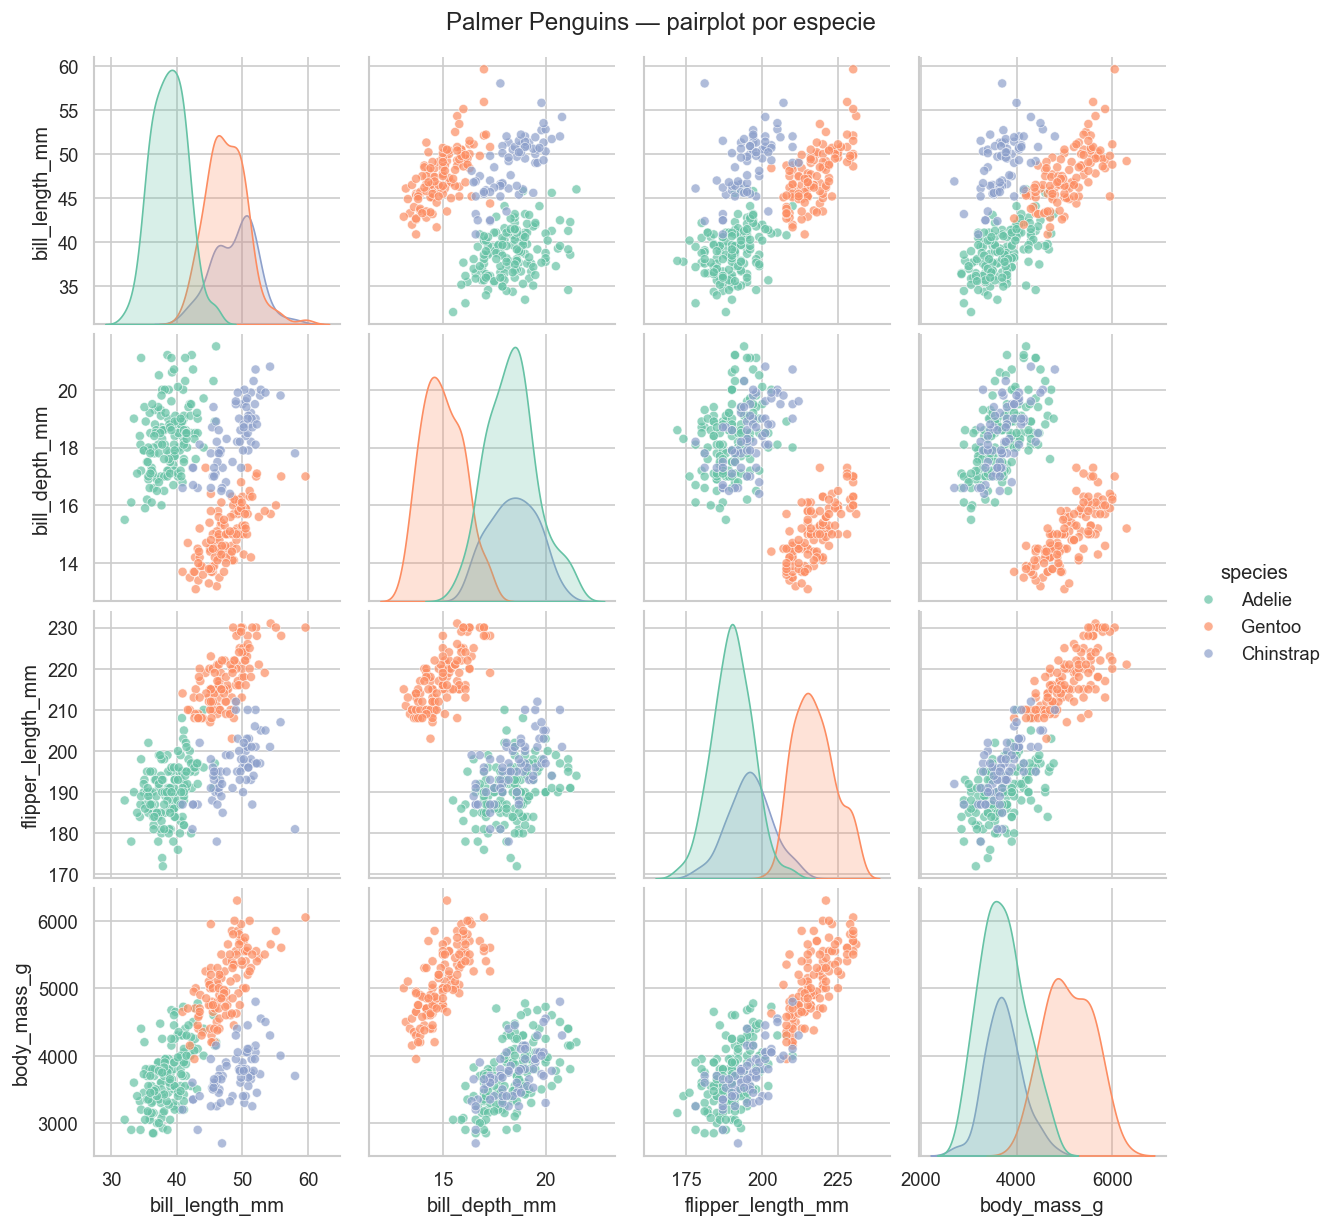
\includegraphics[width=0.98\linewidth]{images/pairplot.png}
\caption{\emph{Pairplot} de las cuatro variables morfométricas discriminado por especie. \emph{Gentoo} se separa claramente del par \emph{Adelie}/\emph{Chinstrap}, especialmente en \texttt{flipper\_length\_mm} y \texttt{body\_mass\_g}. \emph{Adelie} y \emph{Chinstrap} comparten masa corporal y longitud de aleta similares, pero se distinguen por la longitud del pico.}
\label{fig:pairplot}
\end{figure}

\begin{figure}[H]
\centering
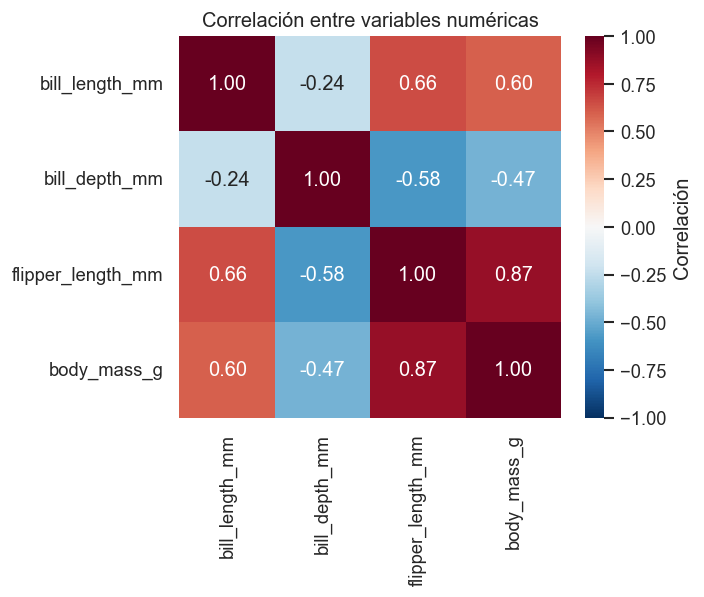
\includegraphics[width=0.62\linewidth]{images/correlacion.png}
\caption{Matriz de correlación de Pearson entre las variables numéricas. La correlación más fuerte se da entre \texttt{flipper\_length\_mm} y \texttt{body\_mass\_g} ($\rho \approx 0.87$). La correlación negativa de $-0.58$ entre \texttt{bill\_depth\_mm} y \texttt{flipper\_length\_mm} es una manifestación de la paradoja de Simpson causada por la mezcla de especies.}
\label{fig:corr}
\end{figure}

\subsection{Determinación del número de clusters}

Antes de fijar $k=3$ se aplicó el \emph{método del codo} para K-Means barriendo $k\in\{1,\dots,8\}$. La figura~\ref{fig:codo} muestra la inercia decreciente con un quiebre visible en $k=3$, congruente con la presencia de tres especies en el dataset.

\begin{figure}[H]
\centering
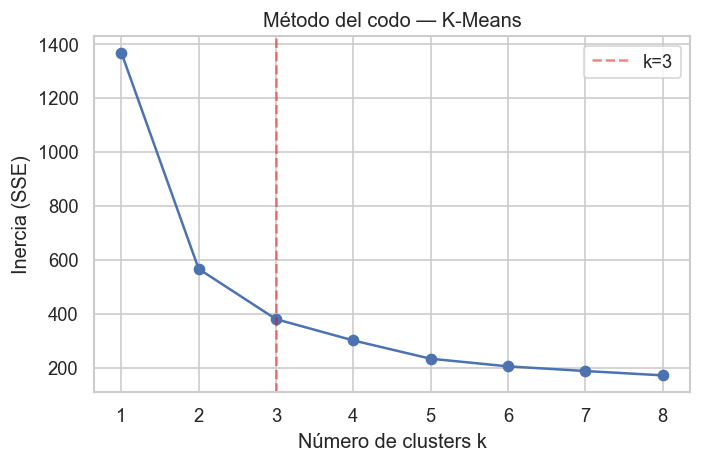
\includegraphics[width=0.62\linewidth]{images/codo.png}
\caption{Método del codo para K-Means sobre las variables estandarizadas. El descenso de la inercia presenta un quiebre en $k=3$.}
\label{fig:codo}
\end{figure}

\subsection{Configuración de los algoritmos}

La tabla~\ref{tab:hyper} consigna los hiperparámetros utilizados; todos los demás se dejan en los valores por omisión de \texttt{scikit-learn}. La semilla \texttt{RANDOM\_STATE} = 42 aplica a K-Means; DBSCAN y Agglomerative son deterministas.

\begin{table}[H]
\centering
\caption{Hiperparámetros de los algoritmos comparados.}
\label{tab:hyper}
\begin{tabularx}{\textwidth}{l >{\hsize=0.85\hsize\raggedright\arraybackslash}X >{\hsize=1.15\hsize\raggedright\arraybackslash}X}
\toprule
\textbf{Algoritmo} & \textbf{Hiperparámetros} & \textbf{Justificación}\\
\midrule
K-Means       & \texttt{n\_clusters=3}, \texttt{n\_init=10}                & $k=3$ por método del codo y por la verdad biológica.\\
DBSCAN        & \texttt{eps=0.6}, \texttt{min\_samples=5}                  & Valor por defecto típico tras estandarización; sin búsqueda fina.\\
Agglomerative & \texttt{n\_clusters=3}, \texttt{linkage="ward"}            & Ward favorece clusters compactos y de varianza homogénea.\\
\bottomrule
\end{tabularx}
\end{table}

% !TEX root = ../main.tex
\section{Resultados}

\subsection{Métricas comparativas}

La tabla~\ref{tab:resultados} reporta el Silhouette Score y el Adjusted Rand Index obtenidos por cada algoritmo sobre las 333 observaciones limpias. Los valores son reproducibles a partir del notebook con \texttt{RANDOM\_STATE} = 42.

\begin{table}[H]
\centering
\caption{Métricas de clustering --- mayor es mejor en ambas columnas.}
\label{tab:resultados}
\begin{tabularx}{0.85\textwidth}{l c c c}
\toprule
\textbf{Algoritmo} & \textbf{Silhouette} & \textbf{ARI} & \textbf{Ruido}\\
\midrule
K-Means                            & 0.447 & 0.793 & 0\\
DBSCAN                             & \textbf{0.557} & 0.584 & 33\\
Agglomerative (\emph{Ward})        & 0.454 & \textbf{0.916} & 0\\
\bottomrule
\end{tabularx}
\end{table}

\subsection{Visualización de los clusters}

La figura~\ref{fig:pca} muestra la proyección PCA bidimensional. La primera componente captura el grueso de la varianza ($\approx 88\%$ entre PC1 y PC2). El panel \emph{Etiqueta verdadera} se incluye como referencia visual: nótese cómo \emph{Gentoo} se separa nítidamente y cómo \emph{Adelie} y \emph{Chinstrap} comparten frontera.

\begin{figure}[H]
\centering
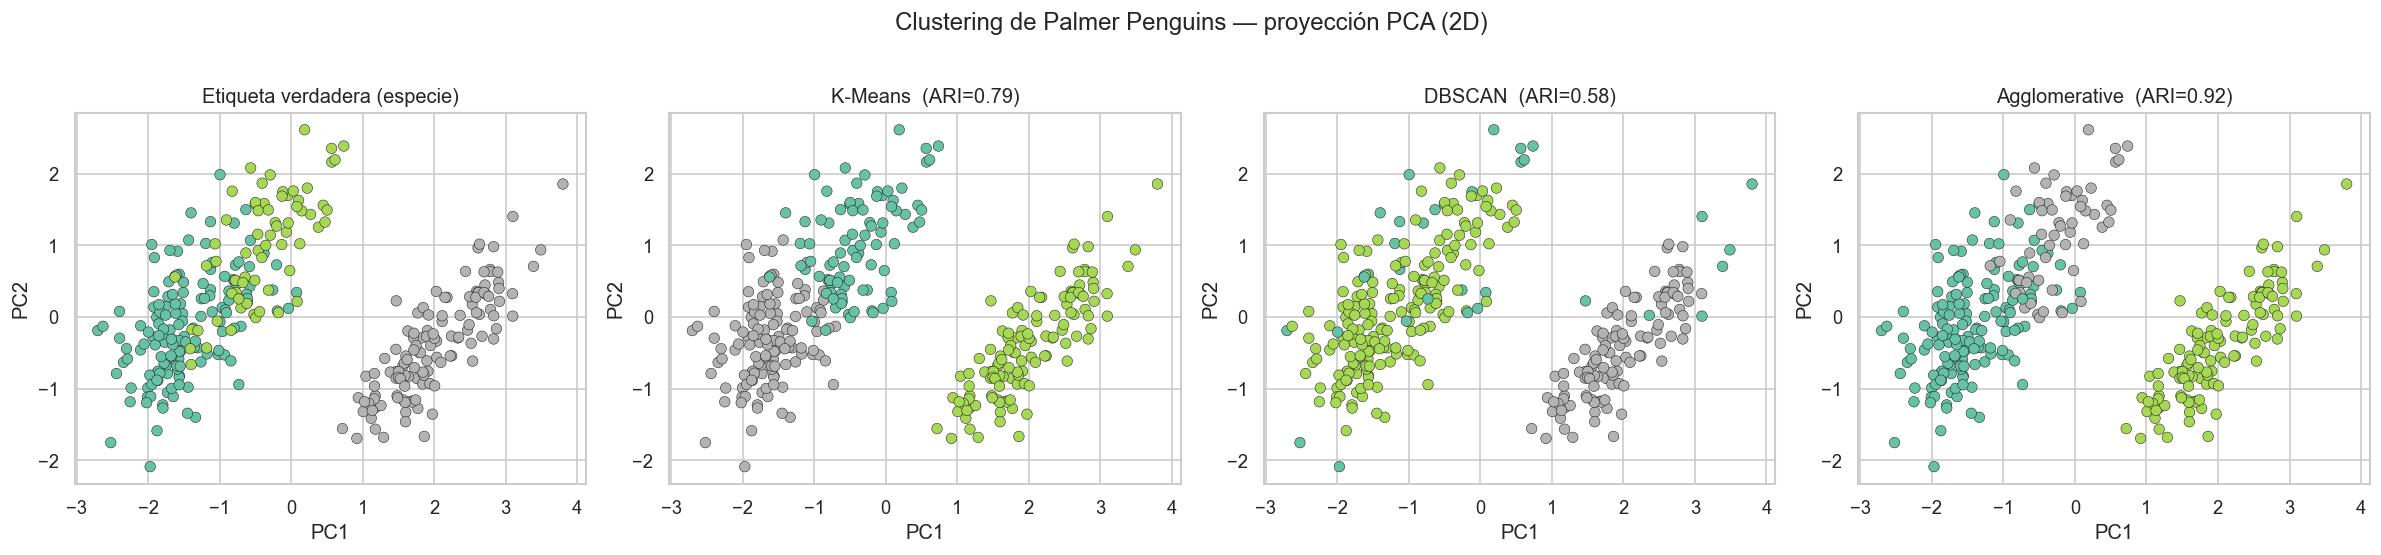
\includegraphics[width=\linewidth]{images/clusters_pca.png}
\caption{Proyección PCA 2D de las 333 observaciones. De izquierda a derecha: etiqueta verdadera de especie, K-Means, DBSCAN y Agglomerative. El ARI consignado en el título de cada panel corresponde al modelo correspondiente.}
\label{fig:pca}
\end{figure}

\subsection{Matriz de confusión del mejor modelo}

Dado que Agglomerative obtiene el mayor ARI, se reporta su matriz de confusión contra la verdad de campo. La figura~\ref{fig:confmat} muestra que los clusters numéricos asignados por el algoritmo se corresponden con las tres especies con un error de asignación pequeño concentrado en la frontera \emph{Adelie}/\emph{Chinstrap}.

\begin{figure}[H]
\centering
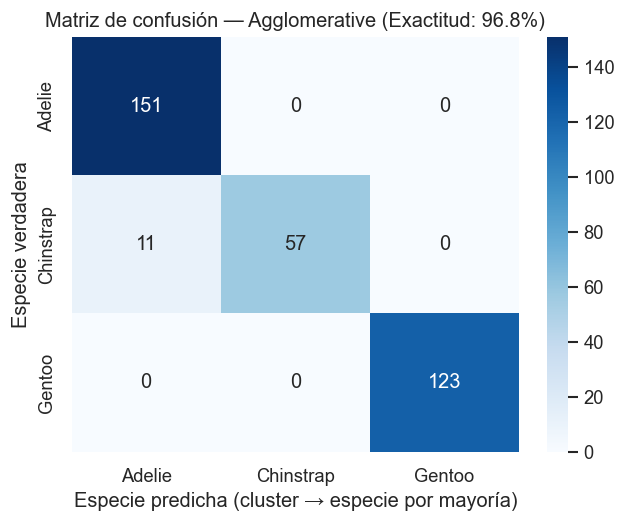
\includegraphics[width=0.6\linewidth]{images/confusion.png}
\caption{Matriz de confusión de Agglomerative Clustering (linkage=Ward) contra la etiqueta verdadera de especie. El emparejamiento cluster--especie es directo y reproduce la estructura biológica.}
\label{fig:confmat}
\end{figure}

\subsection{Discusión}

Los resultados confirman parcialmente la hipótesis. \textbf{Agglomerative} con linkage de Ward es el algoritmo más preciso en términos de ARI (0.916), seguido por \textbf{K-Means} (0.793). Ambos métodos asumen clusters convexos de varianza similar --- supuesto que se cumple razonablemente en este dataset tras estandarización.

\textbf{DBSCAN} obtiene la mejor compacidad interna (Silhouette $=0.557$) porque ignora los 33 puntos marcados como ruido, lo que infla artificialmente la métrica. En la práctica, fusiona \emph{Adelie} y \emph{Chinstrap} en un único cluster denso, hecho que penaliza su ARI. Una búsqueda fina del par $(\varepsilon, \text{minPts})$ mediante la curva $k$-distance \citep{ester1996density,schubert2017dbscan} podría mejorar su desempeño, pero está fuera del alcance de este trabajo corto.

El comportamiento es congruente con la literatura: para datasets pequeños, de baja dimensionalidad y con clusters geométricamente bien separados, los algoritmos centroide-céntricos y jerárquicos suelen superar a los basados en densidad \citep{xu2005survey,saxena2017review}.

% !TEX root = ../main.tex
\section{Conclusiones}

Se aplicó un flujo completo de minería de datos sobre el dataset Palmer Penguins comparando tres algoritmos de clustering no supervisado. La hipótesis inicial --- que algoritmos sensibles a la geometría global recuperarían mejor la estructura biológica que algoritmos basados en densidad --- queda confirmada por las métricas: Agglomerative Clustering con linkage de Ward obtiene un ARI de 0.916 y, tras mapear cada cluster a su especie mayoritaria (Cluster~0~$\to$~\emph{Adelie}, Cluster~1~$\to$~\emph{Gentoo}, Cluster~2~$\to$~\emph{Chinstrap}), una exactitud del 96.8\,\% contra la verdad de campo; K-Means logra ARI 0.793 y DBSCAN, 0.584.

El dataset resultó ideal para el ejercicio docente: tamaño manejable, tres especies bien definidas, presencia controlada de valores faltantes y suficiente solapamiento entre \emph{Adelie} y \emph{Chinstrap} como para que los algoritmos tengan que esforzarse. La estandarización previa de las cuatro variables fue clave; sin ella, \texttt{body\_mass\_g} (en gramos) dominaría las distancias frente a \texttt{bill\_depth\_mm} (en milímetros).

\subsection{Aportes del proyecto}

\begin{itemize}
  \item Notebook reproducible \texttt{notebook.ipynb} ejecutable en Jupyter local y en Google Colab sin pasos manuales.
  \item Comparativa cuantitativa de tres algoritmos con dos métricas complementarias --- interna y externa --- sobre el mismo pipeline.
  \item Cinco figuras vectoriales generadas por el propio notebook: pairplot, matriz de correlación, método del codo, proyección PCA y matriz de confusión.
  \item Presentación PowerPoint (5 diapositivas según rúbrica) generada programáticamente y sincronizada con las métricas del notebook.
  \item Repositorio organizado siguiendo Ciencia 2.0 (README, requirements, datos versionados, semillas fijadas).
\end{itemize}

\subsection{Limitaciones}

\begin{itemize}
  \item Sólo se usaron las cuatro variables numéricas. Las variables categóricas \texttt{sex} e \texttt{island} contienen información discriminante (por ejemplo, las islas de Gentoo y Chinstrap son disjuntas) y podrían mejorar la separación tras encoding.
  \item Los hiperparámetros de DBSCAN se fijaron a un valor estándar; una búsqueda fina con la curva $k$-distance probablemente lo equipararía a K-Means en este dataset.
  \item No se midió la estabilidad de los clusters frente a remuestreo. Un análisis con \emph{bootstrap} reforzaría la validez de los resultados \citep{hennig2007cluster}.
\end{itemize}

\subsection{Trabajo futuro}

Como continuación natural se contemplan: integración de las variables categóricas mediante \emph{one-hot encoding} o \emph{Gower distance}; comparación con Gaussian Mixture Models \citep{mclachlan2000gmm} para clusters elípticos con asignación probabilística; visualización no lineal con UMAP o t-SNE; y validación de estabilidad con \emph{bootstrap} y el índice de Jaccard \citep{hennig2007cluster}. En un horizonte más amplio, sería interesante replicar la metodología sobre el dataset \emph{Iris} y sobre \emph{Pima Indians Diabetes} para contrastar dominios.

\section*{Checklist de Ciencia 2.0}
\addcontentsline{toc}{section}{Checklist de Ciencia 2.0}

\begin{itemize}
  \item Dataset con licencia abierta (CC-0) y enlace al repositorio oficial.
  \item Código fuente íntegro en el notebook, sin dependencias propietarias.
  \item Semillas aleatorias fijadas (\texttt{RANDOM\_STATE=42}).
  \item \texttt{requirements.txt} con las librerías necesarias y sus versiones mínimas.
  \item Notebook ejecutable de principio a fin sin intervención manual.
  \item Reporte en \LaTeX{} con figuras vectoriales y citas verificables.
  \item Presentación de cinco diapositivas alineada con la rúbrica.
\end{itemize}


\appendix
% !TEX root = ../reporte_final.tex
\section{Apéndice: código fuente esencial}
\label{ap:codigo}

Este apéndice contiene los fragmentos esenciales de Python que reproducen el experimento de principio a fin. El notebook completo se encuentra en \texttt{notebook.ipynb} dentro del repositorio del proyecto.

\subsection{Carga y preprocesamiento}

\begin{lstlisting}[language=Python,caption={Carga, limpieza y estandarización del dataset.}]
import os, urllib.request
import pandas as pd
from sklearn.preprocessing import StandardScaler, LabelEncoder

RANDOM_STATE = 42
NUM_COLS = ["bill_length_mm", "bill_depth_mm",
            "flipper_length_mm", "body_mass_g"]

DATA_URL = ("https://raw.githubusercontent.com/allisonhorst/"
            "palmerpenguins/main/inst/extdata/penguins.csv")
LOCAL_PATH = "data/penguins.csv"

if not os.path.exists(LOCAL_PATH):
    os.makedirs("data", exist_ok=True)
    urllib.request.urlretrieve(DATA_URL, LOCAL_PATH)

df = pd.read_csv(LOCAL_PATH)
df_clean = df.dropna(subset=NUM_COLS + ["species"]).reset_index(drop=True)

X = StandardScaler().fit_transform(df_clean[NUM_COLS])
y_true = LabelEncoder().fit_transform(df_clean["species"])
\end{lstlisting}

% Reservamos espacio para subsection + listing 3 completo, evitando
% que el titulo A.2 quede huerfano al pie de la pagina previa.
\Needspace{28\baselineskip}
\subsection{Comparación de algoritmos}

\begin{lstlisting}[language=Python,caption={Ajuste y evaluación de los tres modelos.}]
import numpy as np
from sklearn.cluster import KMeans, DBSCAN, AgglomerativeClustering
from sklearn.metrics import silhouette_score, adjusted_rand_score

models = {
    "K-Means":       KMeans(n_clusters=3, n_init=10,
                            random_state=RANDOM_STATE),
    "DBSCAN":        DBSCAN(eps=0.6, min_samples=5),
    "Agglomerative": AgglomerativeClustering(n_clusters=3,
                                             linkage="ward"),
}

for name, m in models.items():
    labels = m.fit_predict(X)
    mask = labels != -1
    sil = (silhouette_score(X[mask], labels[mask])
           if len(set(labels[mask])) > 1 else np.nan)
    ari = adjusted_rand_score(y_true, labels)
    n_noise = int((labels == -1).sum())
    print(f"{name:15s}  sil={sil:.3f}  ari={ari:.3f}  ruido={n_noise}")
\end{lstlisting}

% !TEX root = ../main.tex
\section{Apéndice: instrucciones de reproducibilidad}
\label{ap:reproducibilidad}

\subsection{Estructura del repositorio}

\begin{lstlisting}[caption={Disposición de archivos del proyecto.}]
mineria/
+- notebook.ipynb       Notebook principal (Jupyter / Google Colab)
+- README.md            Resumen del proyecto y guia de ejecucion
+- requirements.txt     Dependencias minimas con version
+- data/
|  +- penguins.csv      Dataset Palmer Penguins (CC-0)
+- images/              Figuras vectoriales generadas por el notebook
+- presentacion.pptx    Presentacion de 5 diapositivas
+- report/
   +- main.tex          Reporte LaTeX (este documento)
   +- sections/         Secciones modulares
   +- images/           Copia de figuras para el reporte
   +- references.bib    Bibliografia
\end{lstlisting}

\subsection{Ejecución local}

\begin{lstlisting}[language=bash,caption={Reproducción del experimento en local.}]
git clone <repo-url> mineria
cd mineria
python -m venv venv
venv\Scripts\activate              # Windows (en Linux/Mac: source venv/bin/activate)
pip install -r requirements.txt
jupyter notebook notebook.ipynb
\end{lstlisting}

\subsection{Ejecución en Google Colab}

\begin{enumerate}
  \item Subir \texttt{notebook.ipynb} a Google Drive.
  \item Abrirlo con Google Colab.
  \item Ejecutar \texttt{Entorno de ejecución $\rightarrow$ Ejecutar todo}.
  \item El dataset se descarga automáticamente desde el repositorio oficial si no está disponible localmente.
\end{enumerate}

\subsection{Compilación del reporte LaTeX}

\begin{lstlisting}[language=bash,caption={Compilación del PDF en el directorio report/.}]
cd report
pdflatex main.tex
bibtex main
pdflatex main.tex
pdflatex main.tex
\end{lstlisting}

\subsection{Checklist de Ciencia 2.0}

\begin{itemize}
  \item[\checkmark] Datos abiertos con licencia CC-0 y enlace al repositorio fuente.
  \item[\checkmark] Código abierto en notebook y scripts auxiliares.
  \item[\checkmark] Semillas aleatorias fijadas (\texttt{RANDOM\_STATE} = 42).
  \item[\checkmark] Dependencias declaradas con versiones mínimas (\texttt{requirements.txt}).
  \item[\checkmark] Notebook ejecutable de principio a fin sin pasos manuales.
  \item[\checkmark] Reporte LaTeX y presentación generados a partir de los mismos resultados.
\end{itemize}


% --- Bibliografia ---
% Las penalizaciones globales (clubpenalty/widowpenalty=10000) y el
% raggedbottom hacen que cualquier entrada de 2 lineas que no quepa
% completa se mueva entera a la pagina siguiente, dejando huecos
% grandes al final de pagina. En la bibliografia esto es indeseable
% porque cada \bibitem es un parrafo independiente y es preferible
% que una entrada larga se parta entre paginas a dejar 5+ cm de hueco.
% Solucion: arrancar en pagina nueva, apretar bibsep y permitir que
% las entradas se rompan internamente (penalizaciones bajas localmente).
\clearpage
\begingroup
\setlength{\bibsep}{0.45em plus 0.1em minus 0.05em}
\clubpenalty=150
\widowpenalty=150
\interlinepenalty=0
\raggedbottom
\bibliographystyle{apalike}
\bibliography{references}
\endgroup

\end{document}
